\documentclass{beamer}
\usepackage[utf8]{inputenc}

\usetheme{Goettingen}
\usecolortheme{default}
\usefonttheme{structurebold}
\usepackage{svg}
\usepackage{fancybox}
%------------------------------------------------------------
%This block of code defines the information to appear in the
%Title page
\title[Open Data Game Jam] %optional
{Open Data Game Jam}

%End of title page configuration block
%------------------------------------------------------------



%------------------------------------------------------------
%The next block of commands puts the table of contents at the 
%beginning of each section and highlights the current section:

\AtBeginSection[]
{
  \begin{frame}
    \frametitle{Table of Contents}
    \tableofcontents[currentsection]
  \end{frame}
}
%------------------------------------------------------------


\begin{document}

%The next statement creates the title page.
\frame{\titlepage}


%---------------------------------------------------------
%This block of code is for the table of contents after
%the title page
\begin{frame}
\frametitle{Table of Contents}
\tableofcontents
\end{frame}
%---------------------------------------------------------


\section{Introduction}

%---------------------------------------------------------
%Changing visivility of the text
\begin{frame}
\frametitle{Facilitator}
Short introduction from the facilitator
\end{frame}

%---------------------------------------------------------


%---------------------------------------------------------
\begin{frame}
\frametitle{Assistant}
Short introduction from the assistant
\end{frame}
%---------------------------------------------------------

%---------------------------------------------------------
\begin{frame}
\frametitle{Objectives}
\begin{itemize}
    \item Express a social issues through a video game (prototype)
    \item Reflect on available open data
    \item Have fun
    \item Learn something new
\end{itemize}
\end{frame}
%---------------------------------------------------------

%---------------------------------------------------------
\begin{frame}
\frametitle{Spent}
\begin{figure}
 \shadowbox{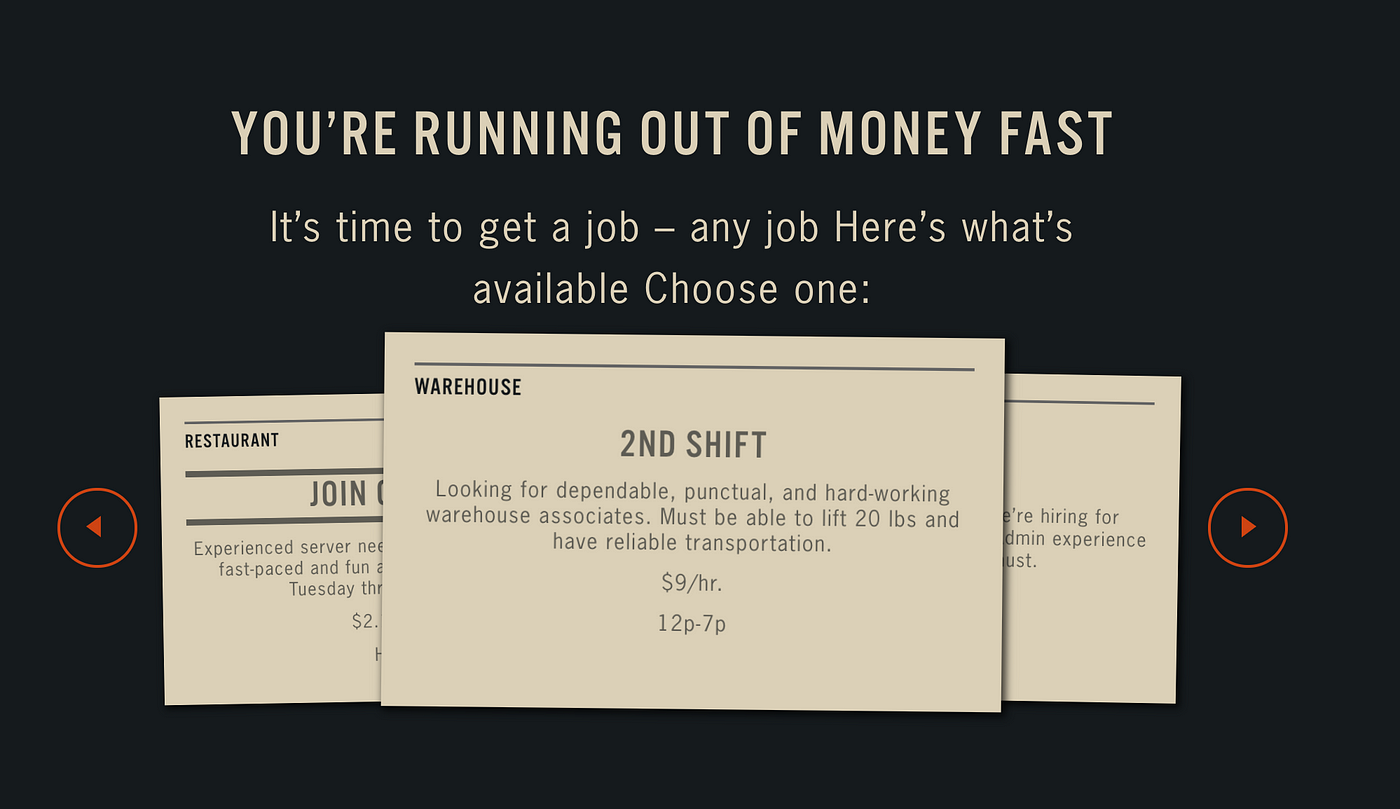
\includegraphics[width=.9\textwidth]{figures/spent.png}}
\end{figure}
\end{frame}
%---------------------------------------------------------
\begin{frame}
\frametitle{McDonald's videogame}
\begin{figure}
 \shadowbox{\includegraphics[width=.9\textwidth]{figures/mcdonalds.png}}
\end{figure}
\end{frame}
%---------------------------------------------------------
%---------------------------------------------------------
\begin{frame}
\frametitle{Duolingo}
\begin{figure}
 \shadowbox{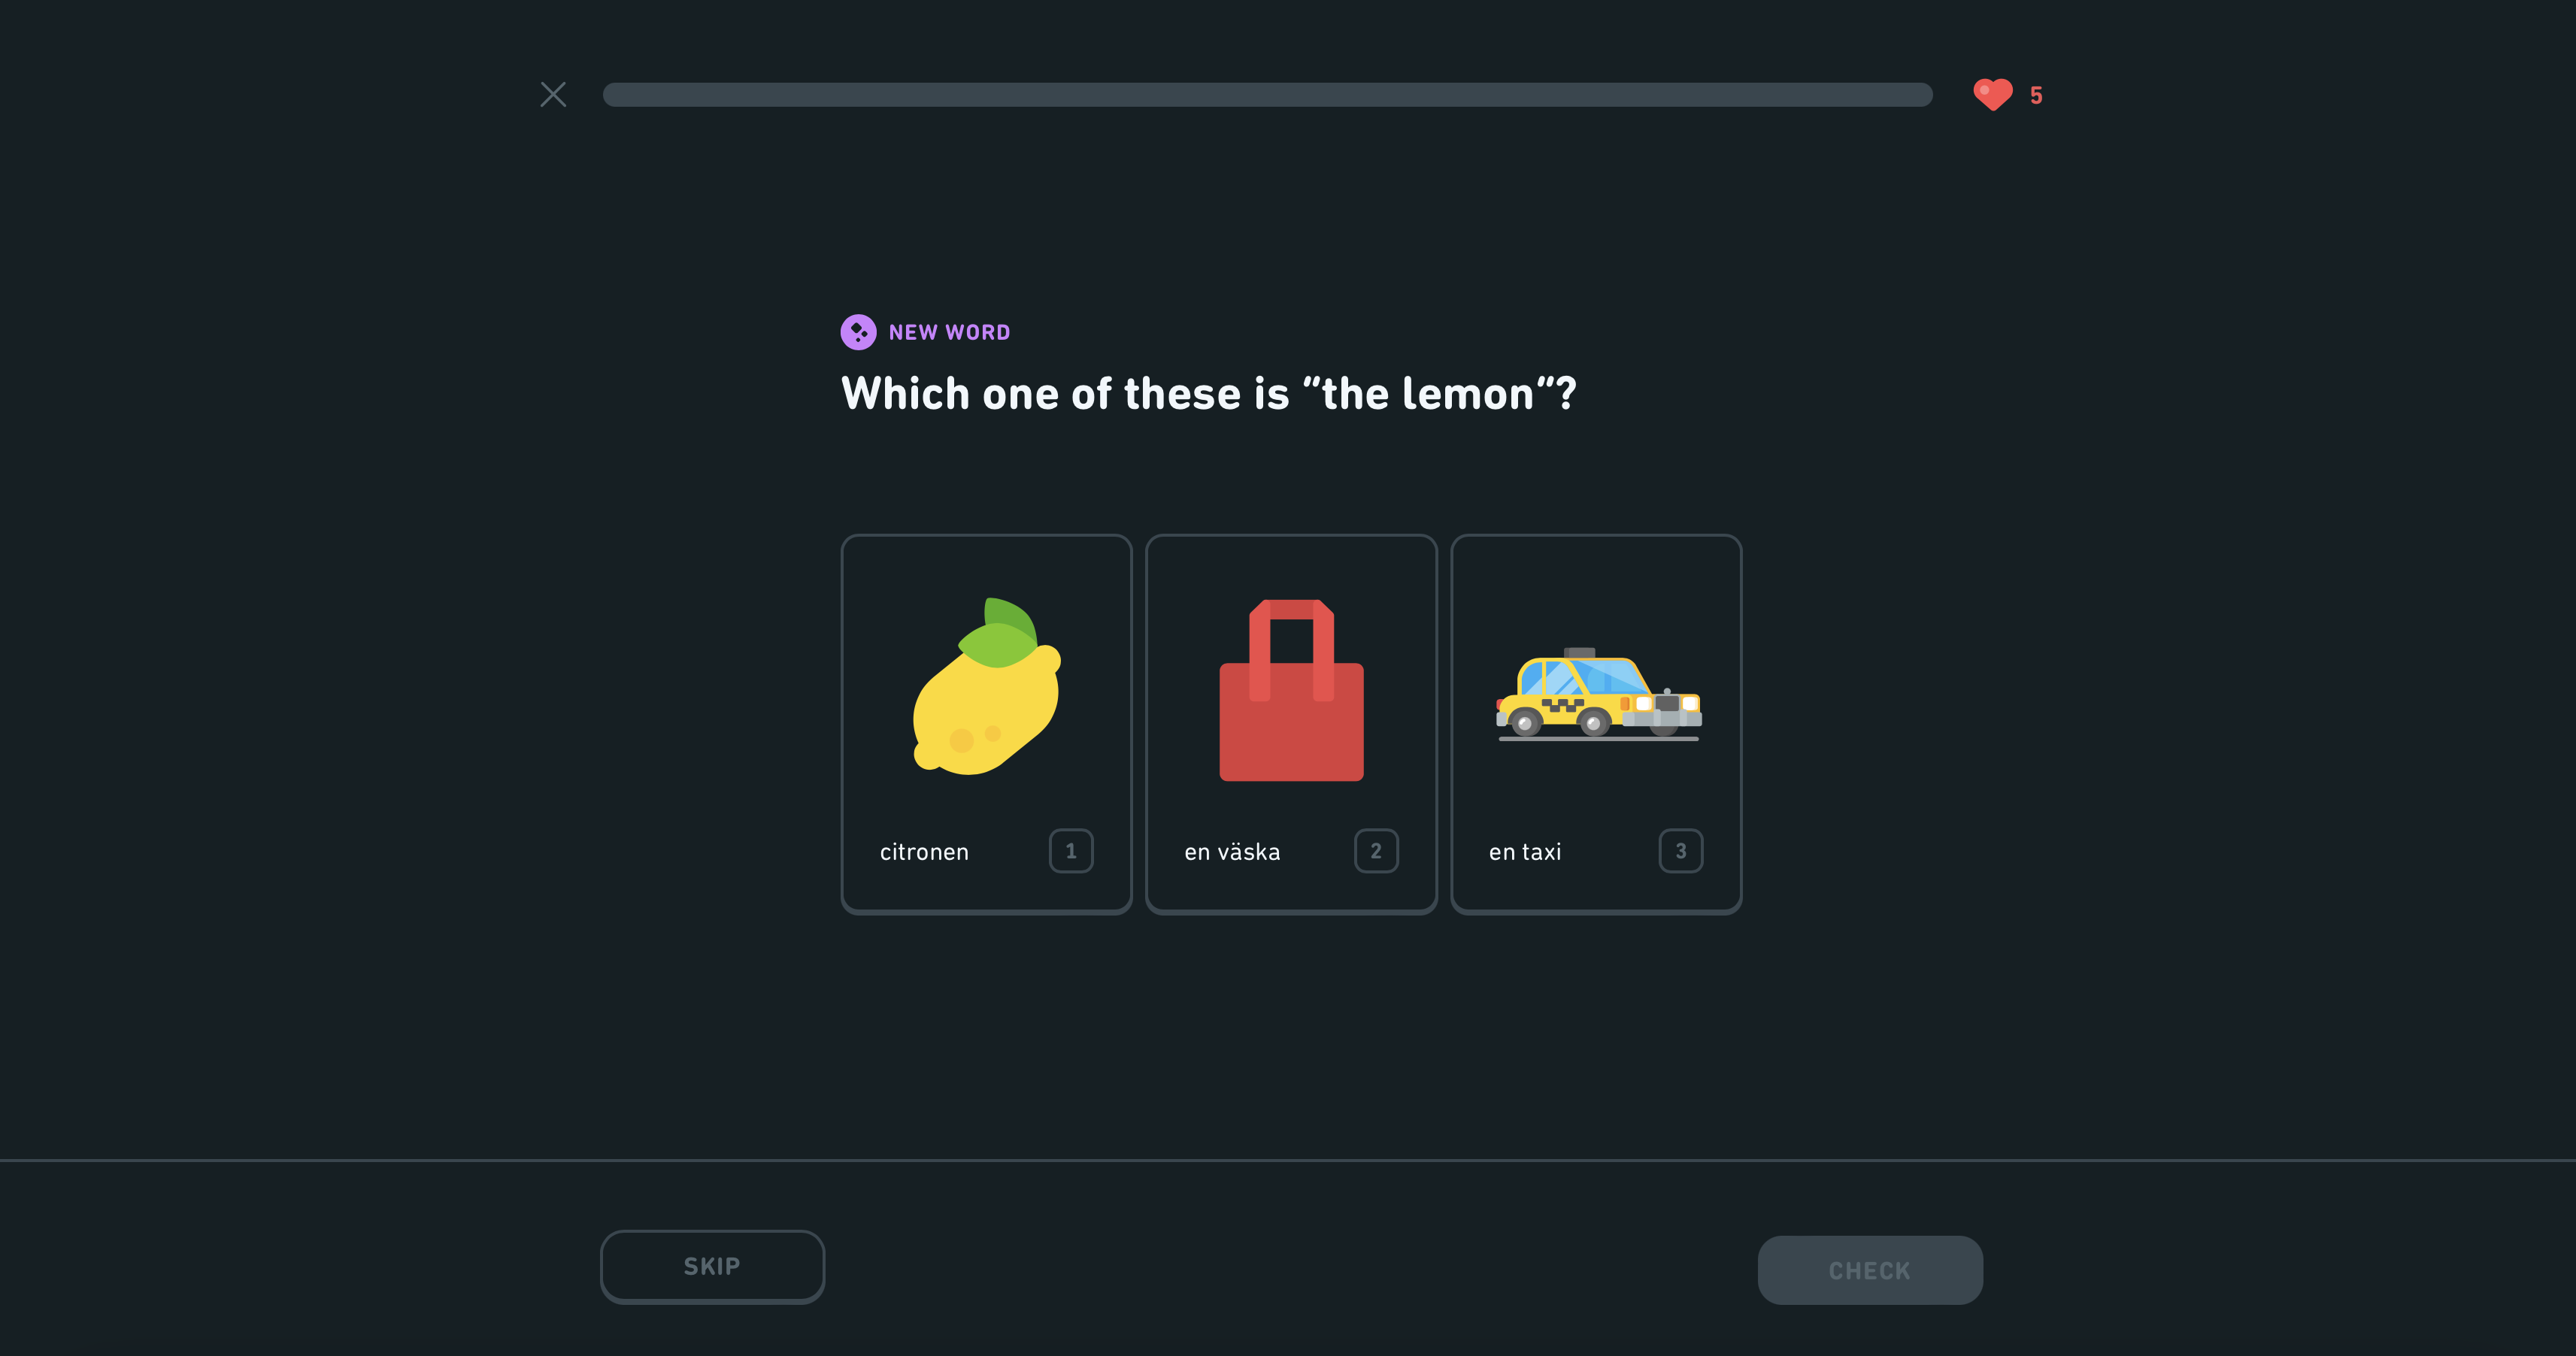
\includegraphics[width=.9\textwidth]{figures/duolingo.png}}
\end{figure}
\end{frame}

\begin{frame}
\frametitle{You don't need to be amazing at this}
Some examples from develop.games
\end{frame}

\begin{frame}
\frametitle{You don't need to be an amazing artist}
\begin{figure}
 \shadowbox{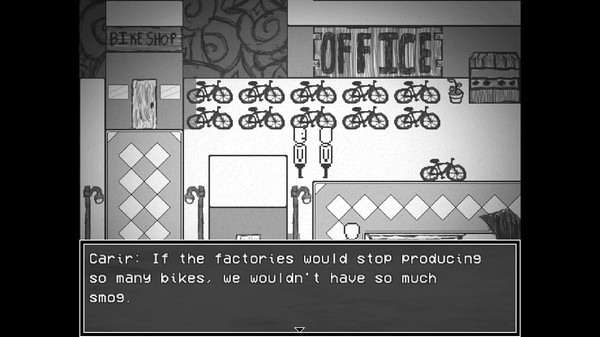
\includegraphics[width=.9\textwidth]{figures/suits.jpg}}
\end{figure}
\end{frame}

\begin{frame}
\frametitle{You don't need to be an amazing sound designer}
\begin{figure}
 \shadowbox{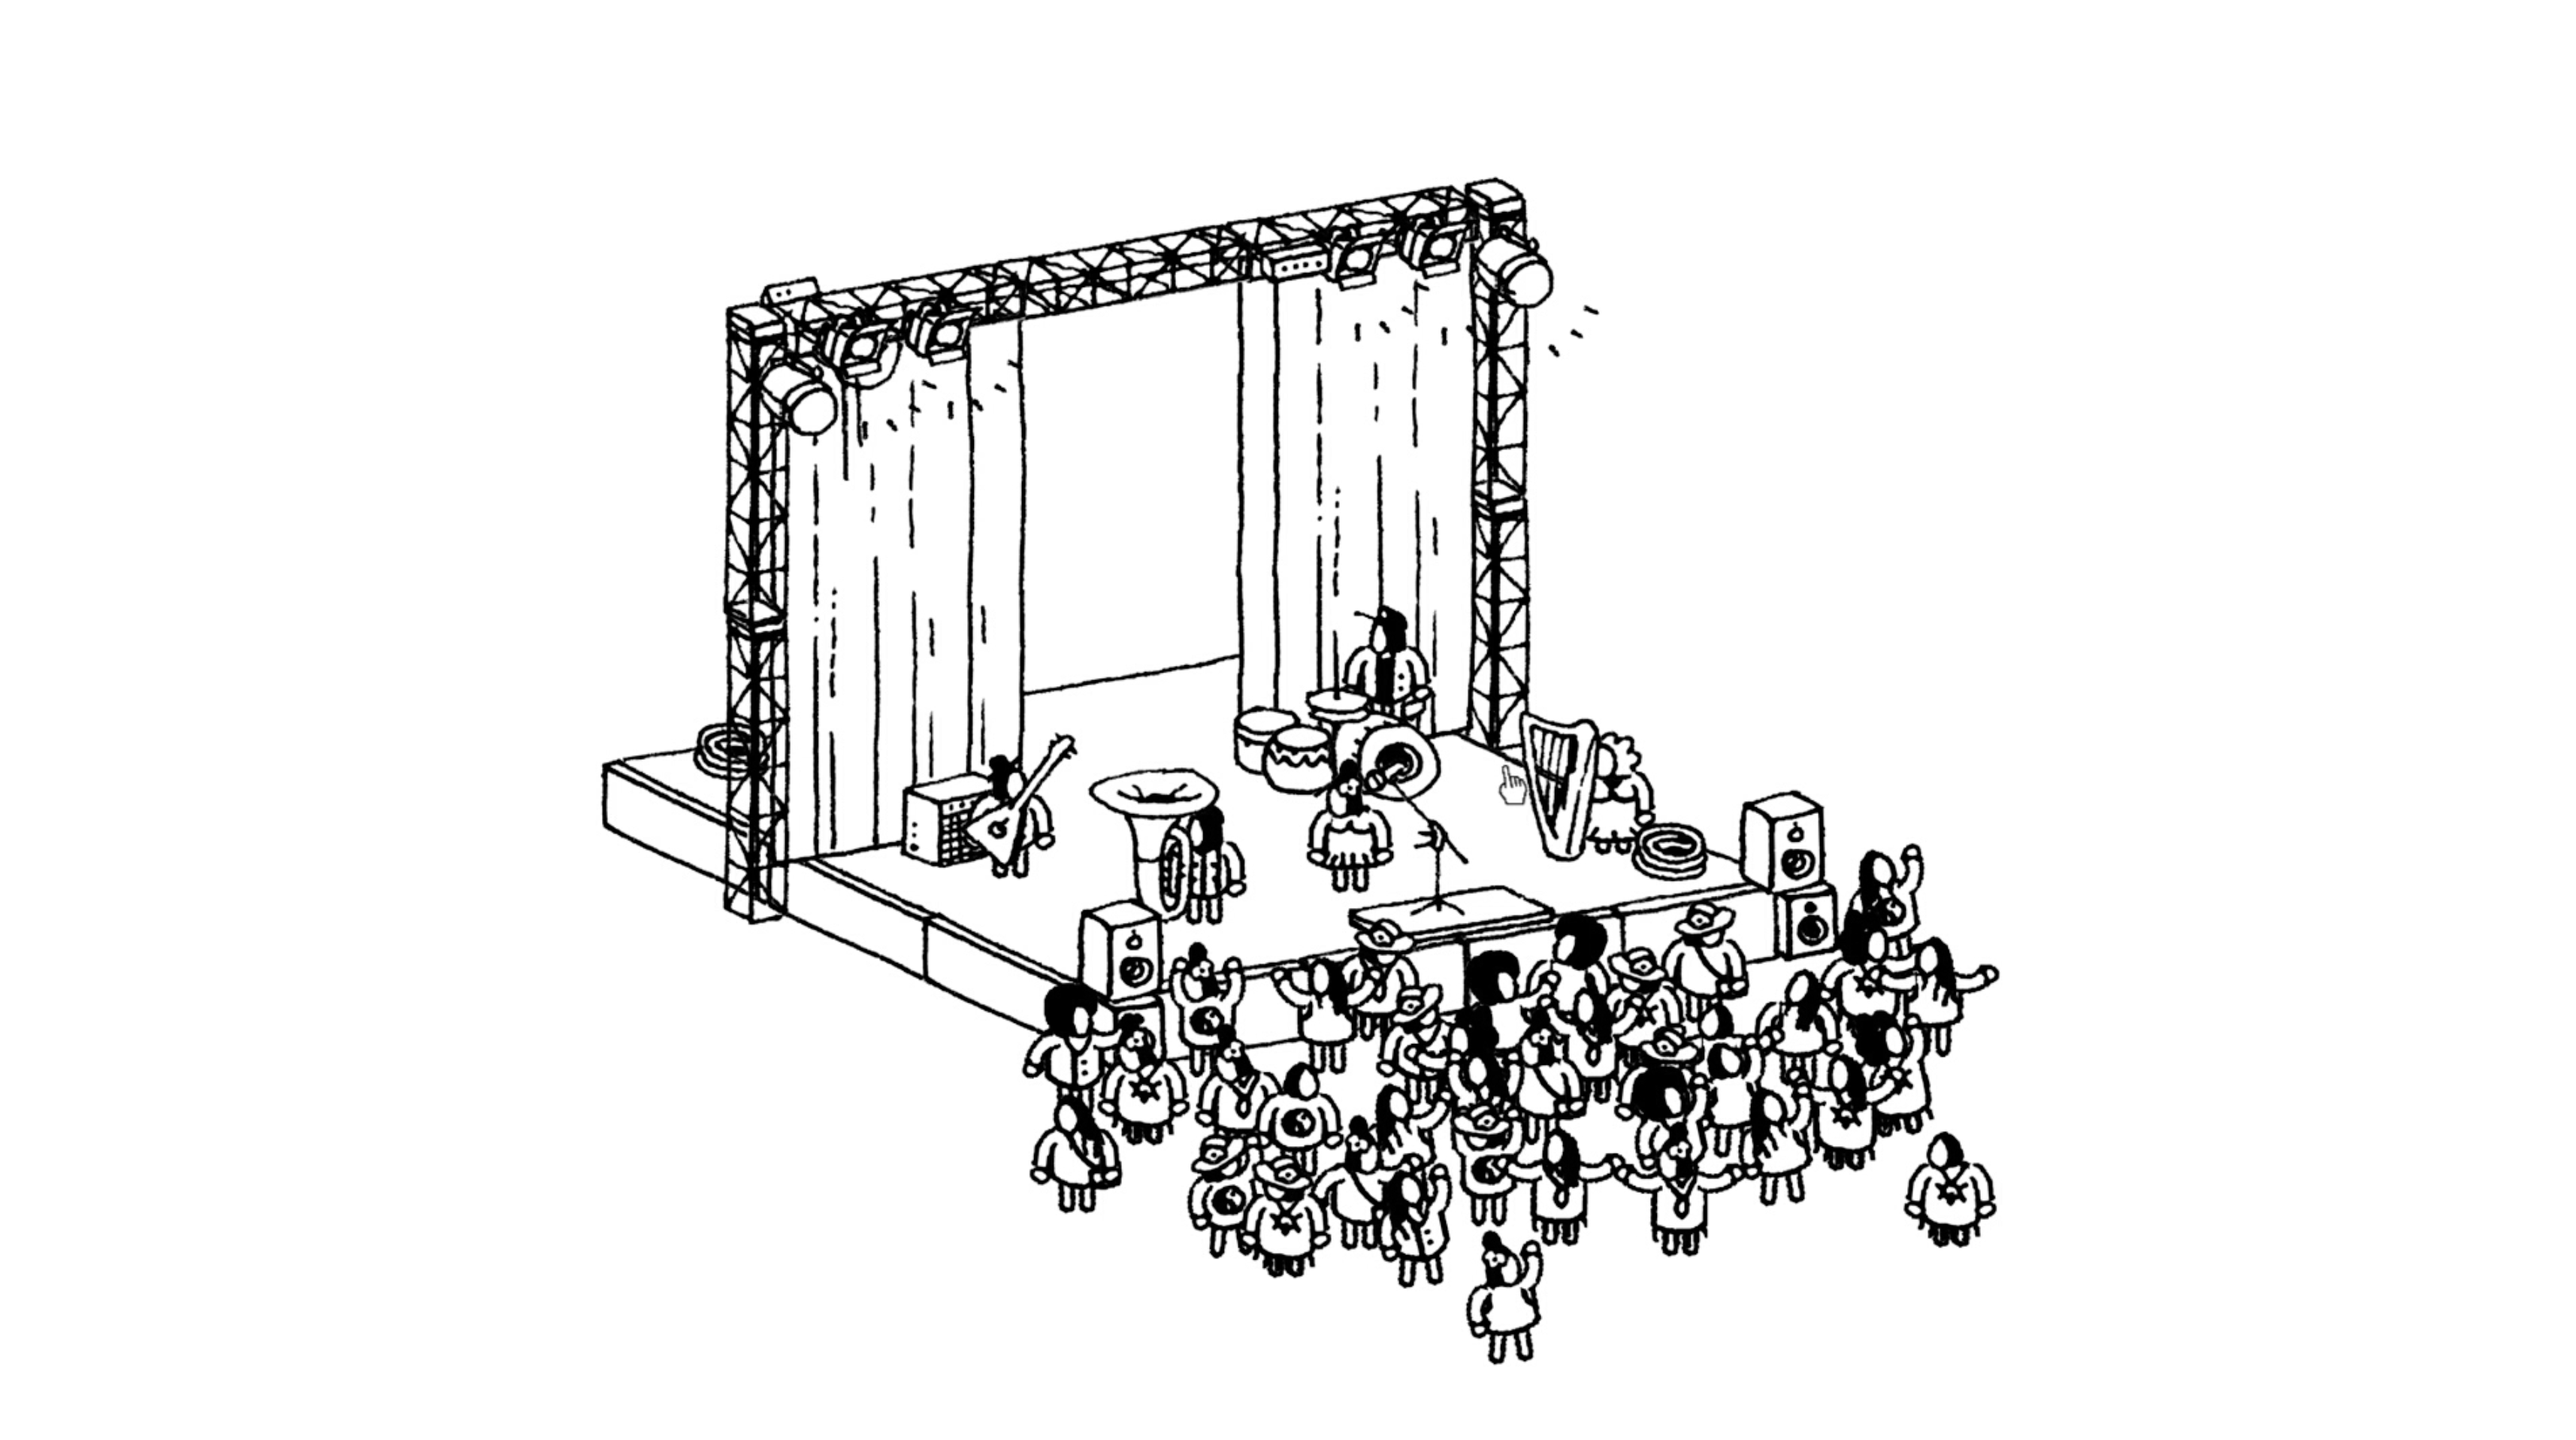
\includegraphics[width=.9\textwidth]{figures/hidden_folks.png}}
\end{figure}
\end{frame}

\begin{frame}
\frametitle{You don't need to be an amazing coder}
\begin{figure}
 \shadowbox{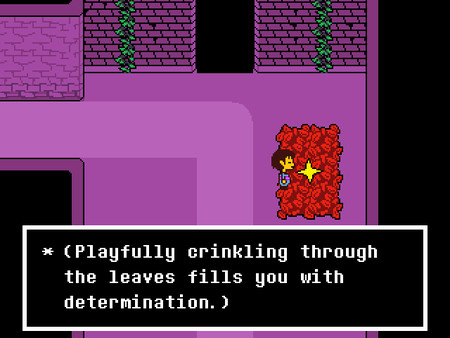
\includegraphics[width=.9\textwidth]{figures/undertale.jpg}}
\end{figure}
\end{frame}

\begin{frame}
\frametitle{You don't need to be an amazing coder}
\begin{figure}
 \shadowbox{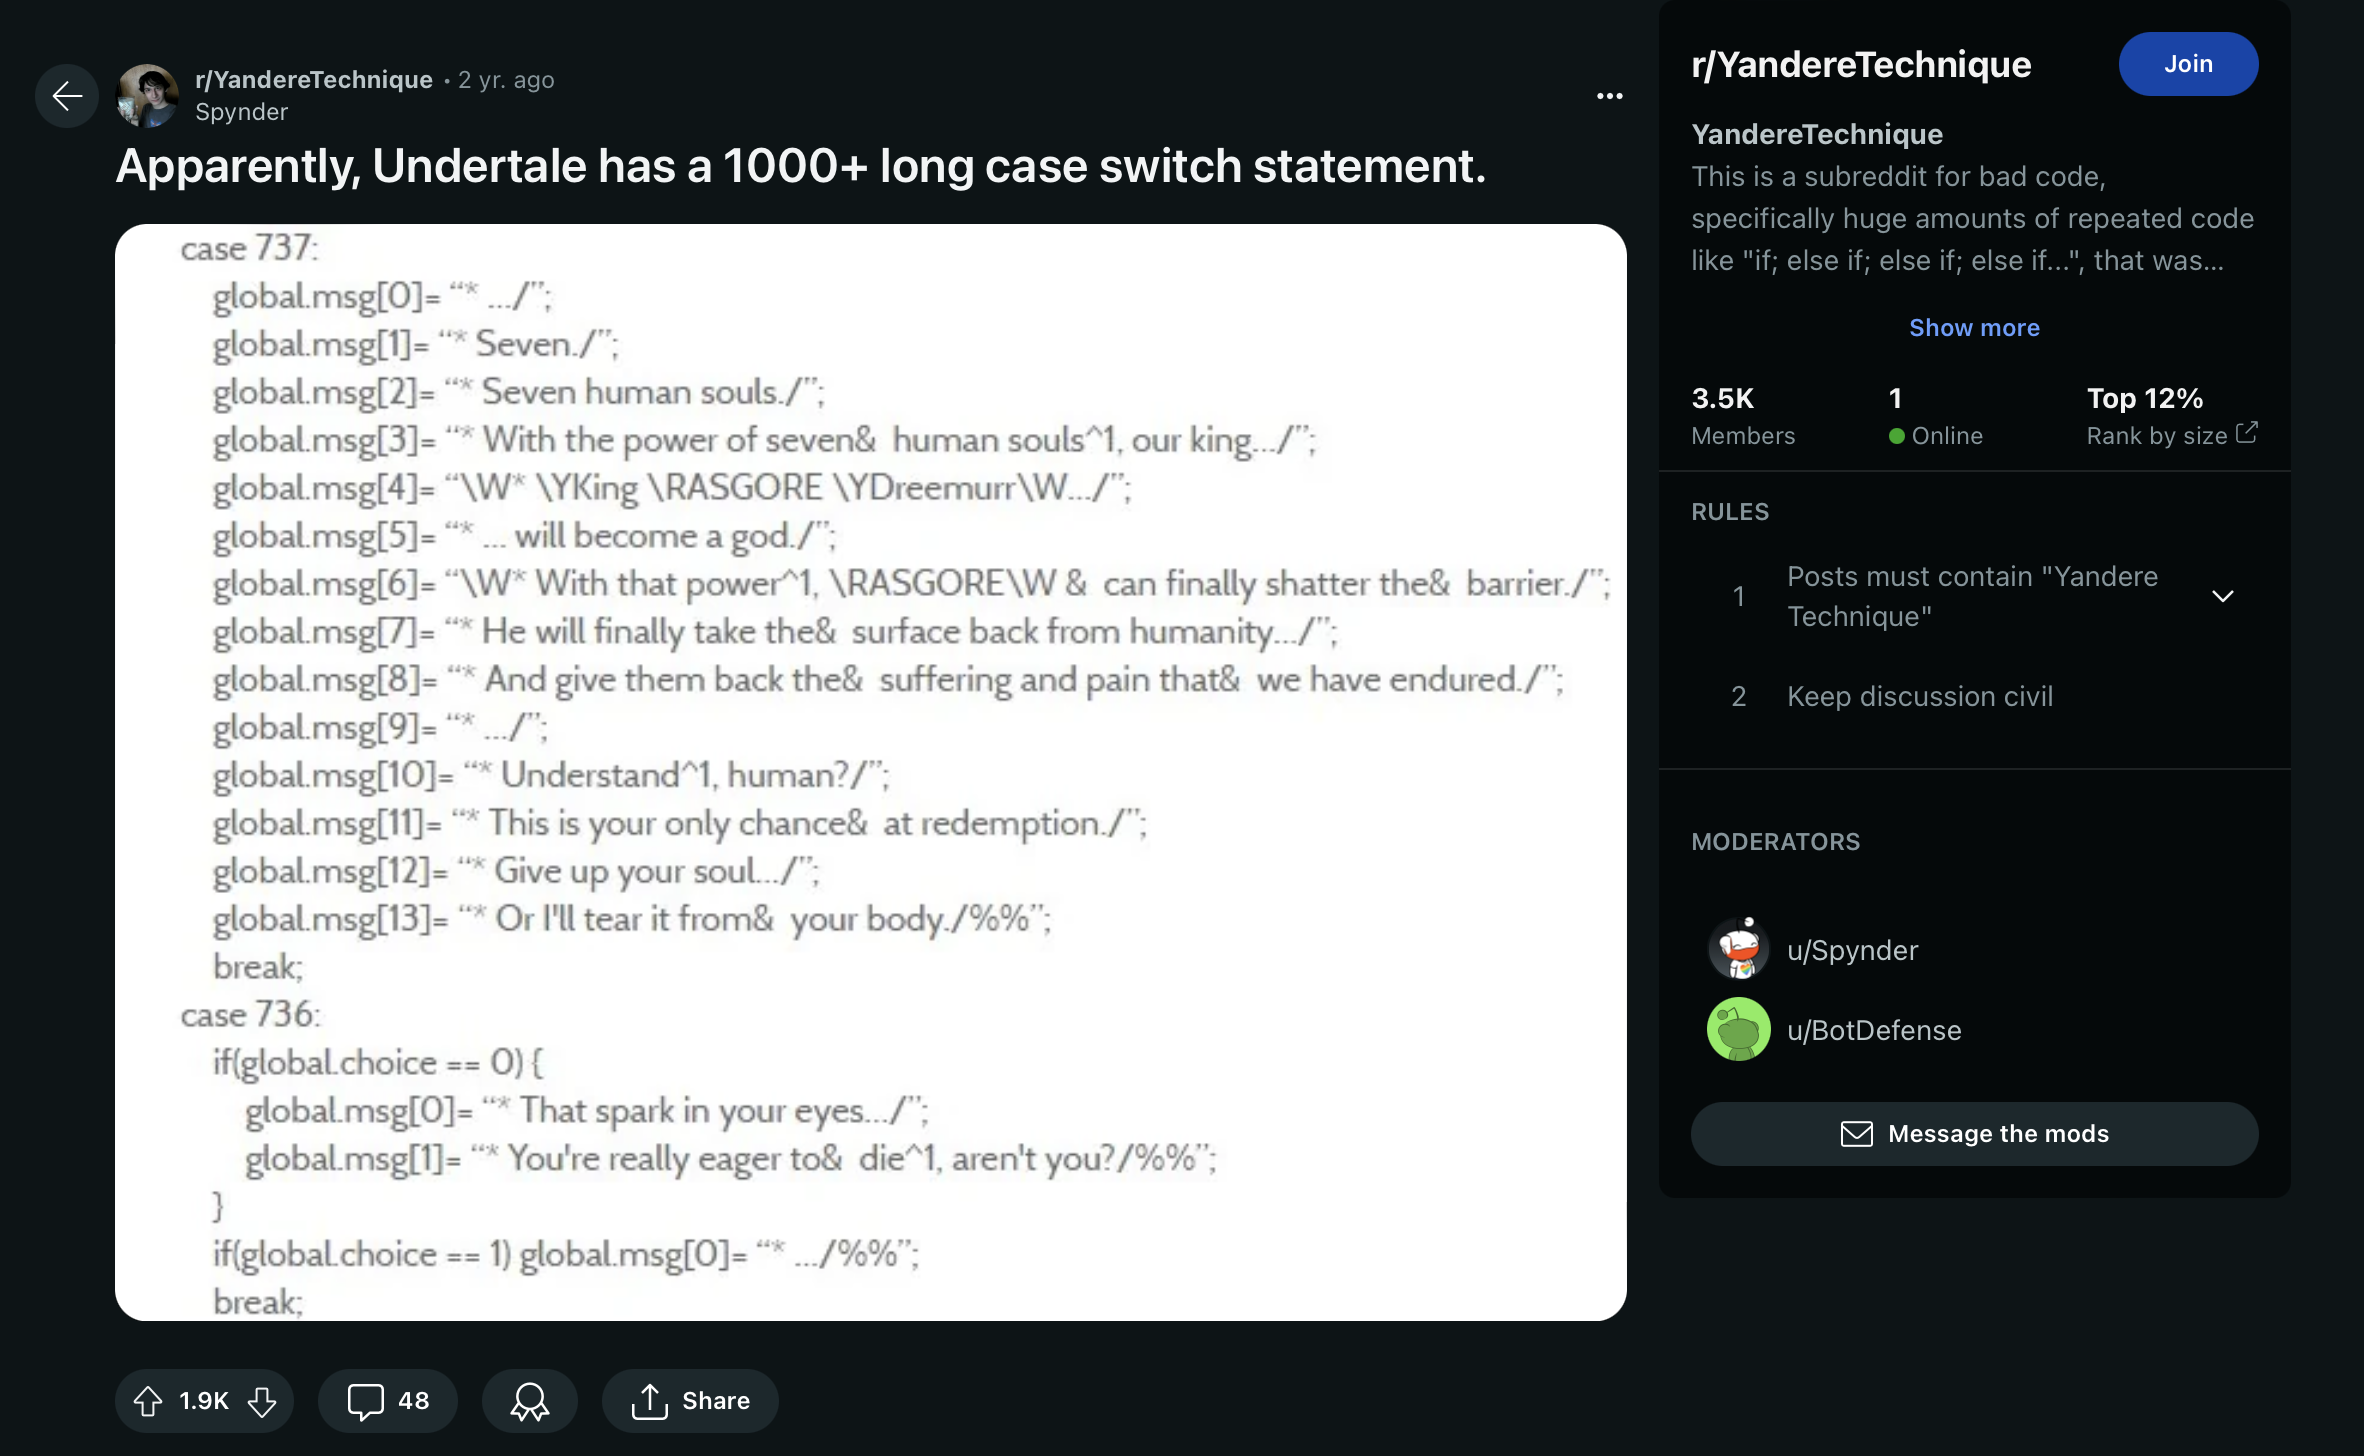
\includegraphics[width=.9\textwidth]{figures/undertale_code.png}}
\end{figure}
\end{frame}


\section{Icebreaker}
\begin{frame}
\frametitle{Human Bingo}
\begin{figure}
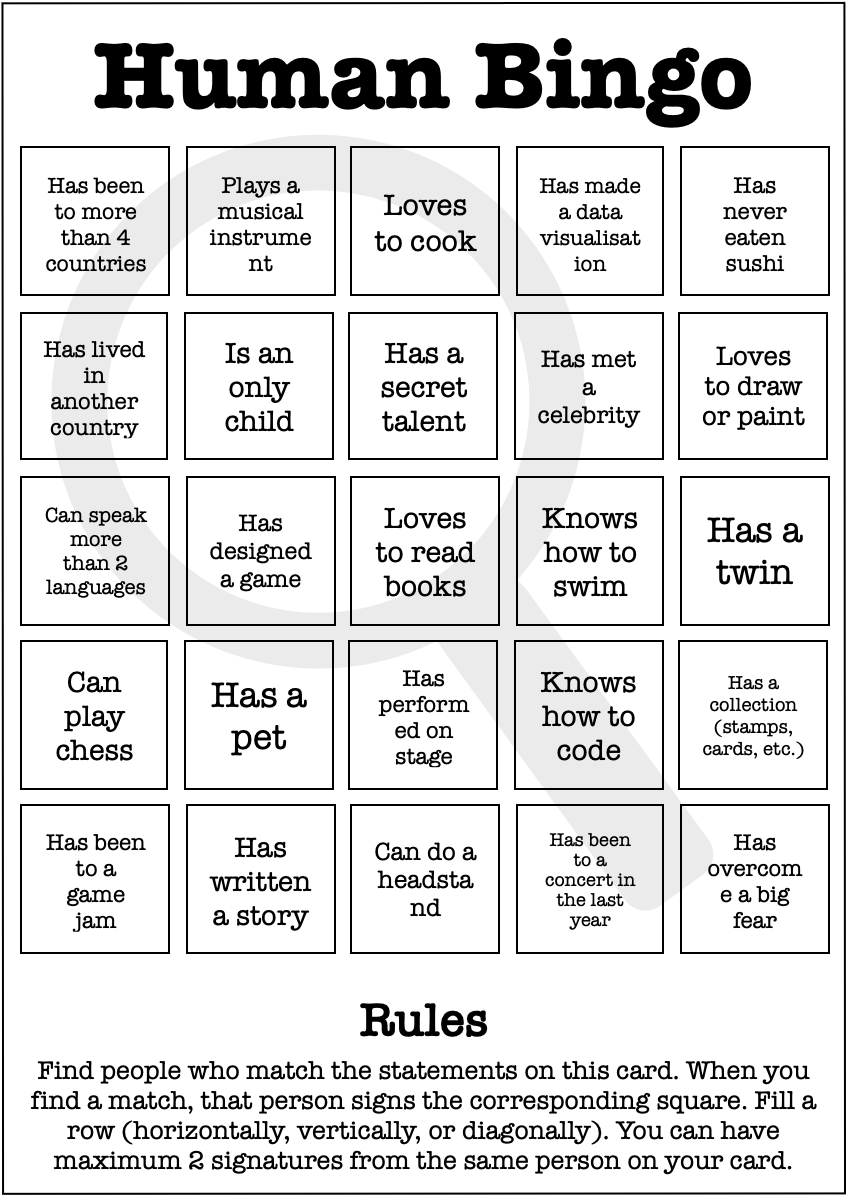
\includegraphics[width=.8\textwidth, angle=10]{figures/human_bingo.png}
\end{figure}
\end{frame}



\section{Make your badge}
\begin{frame}
\frametitle{Pick an empty badge}
\begin{itemize}
    \item Stickers available: Artist, Game designer, Issue expert, Coder
    \item You can write something else if you like!
    \item Wear it: make a string, clip it, or in any other way
\end{itemize}
\begin{figure}
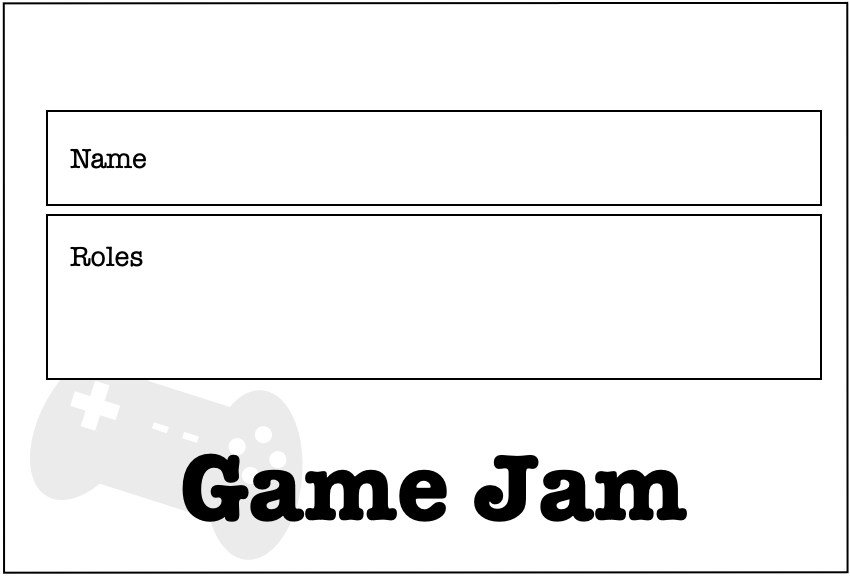
\includegraphics[width=0.9\textwidth, angle=10]{figures/badge.png}
\end{figure}
\end{frame}

\section{Issue brainstorming}
\begin{frame}
\frametitle{Issue pitch sheet}
Take a sheet if you want to propose an idea
\begin{figure}
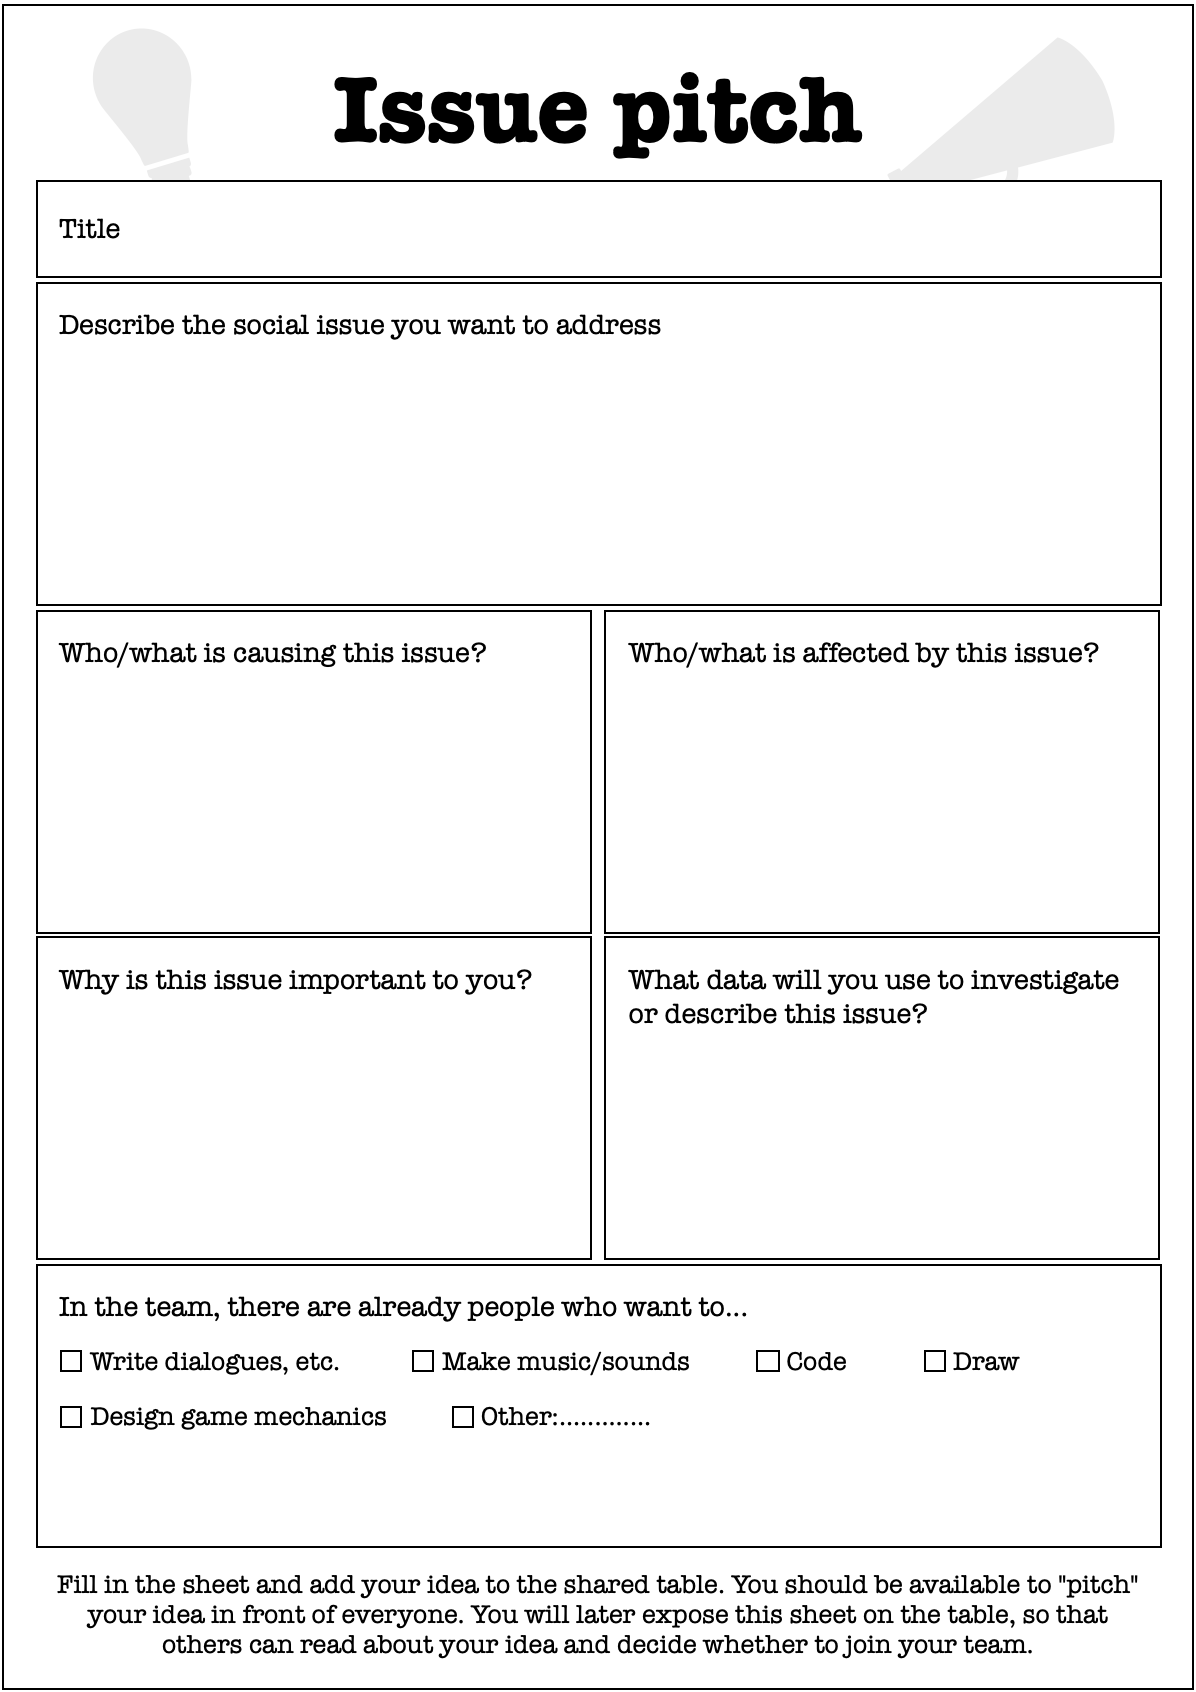
\includegraphics[width=0.9\textwidth, angle=10]{figures/issue_pitch.png}
\end{figure}
\end{frame}

\section{Pitches}
\begin{frame}
\frametitle{Time to present!}
Max 2', don't forget to mention:
\begin{itemize}
    \item Why the issue is important to you
    \item Data available
    \item Skills needed in your team
\end{itemize}
\begin{figure}
\includesvg[width=0.8\textwidth]{figures/pitching.svg}
\end{figure}
\end{frame}

\section{Group formation}
\begin{frame}
\frametitle{Group formation}
Divide into groups of 4
\begin{figure}
\includesvg[width=0.8\textwidth]{figures/network.svg}
\end{figure}
\end{frame}

\section{Survey section 1}
\begin{frame}
\frametitle{Survey section 1}
Fill until the end of section 1, then keep the survey with you until the end of the event
\begin{figure}
 \shadowbox{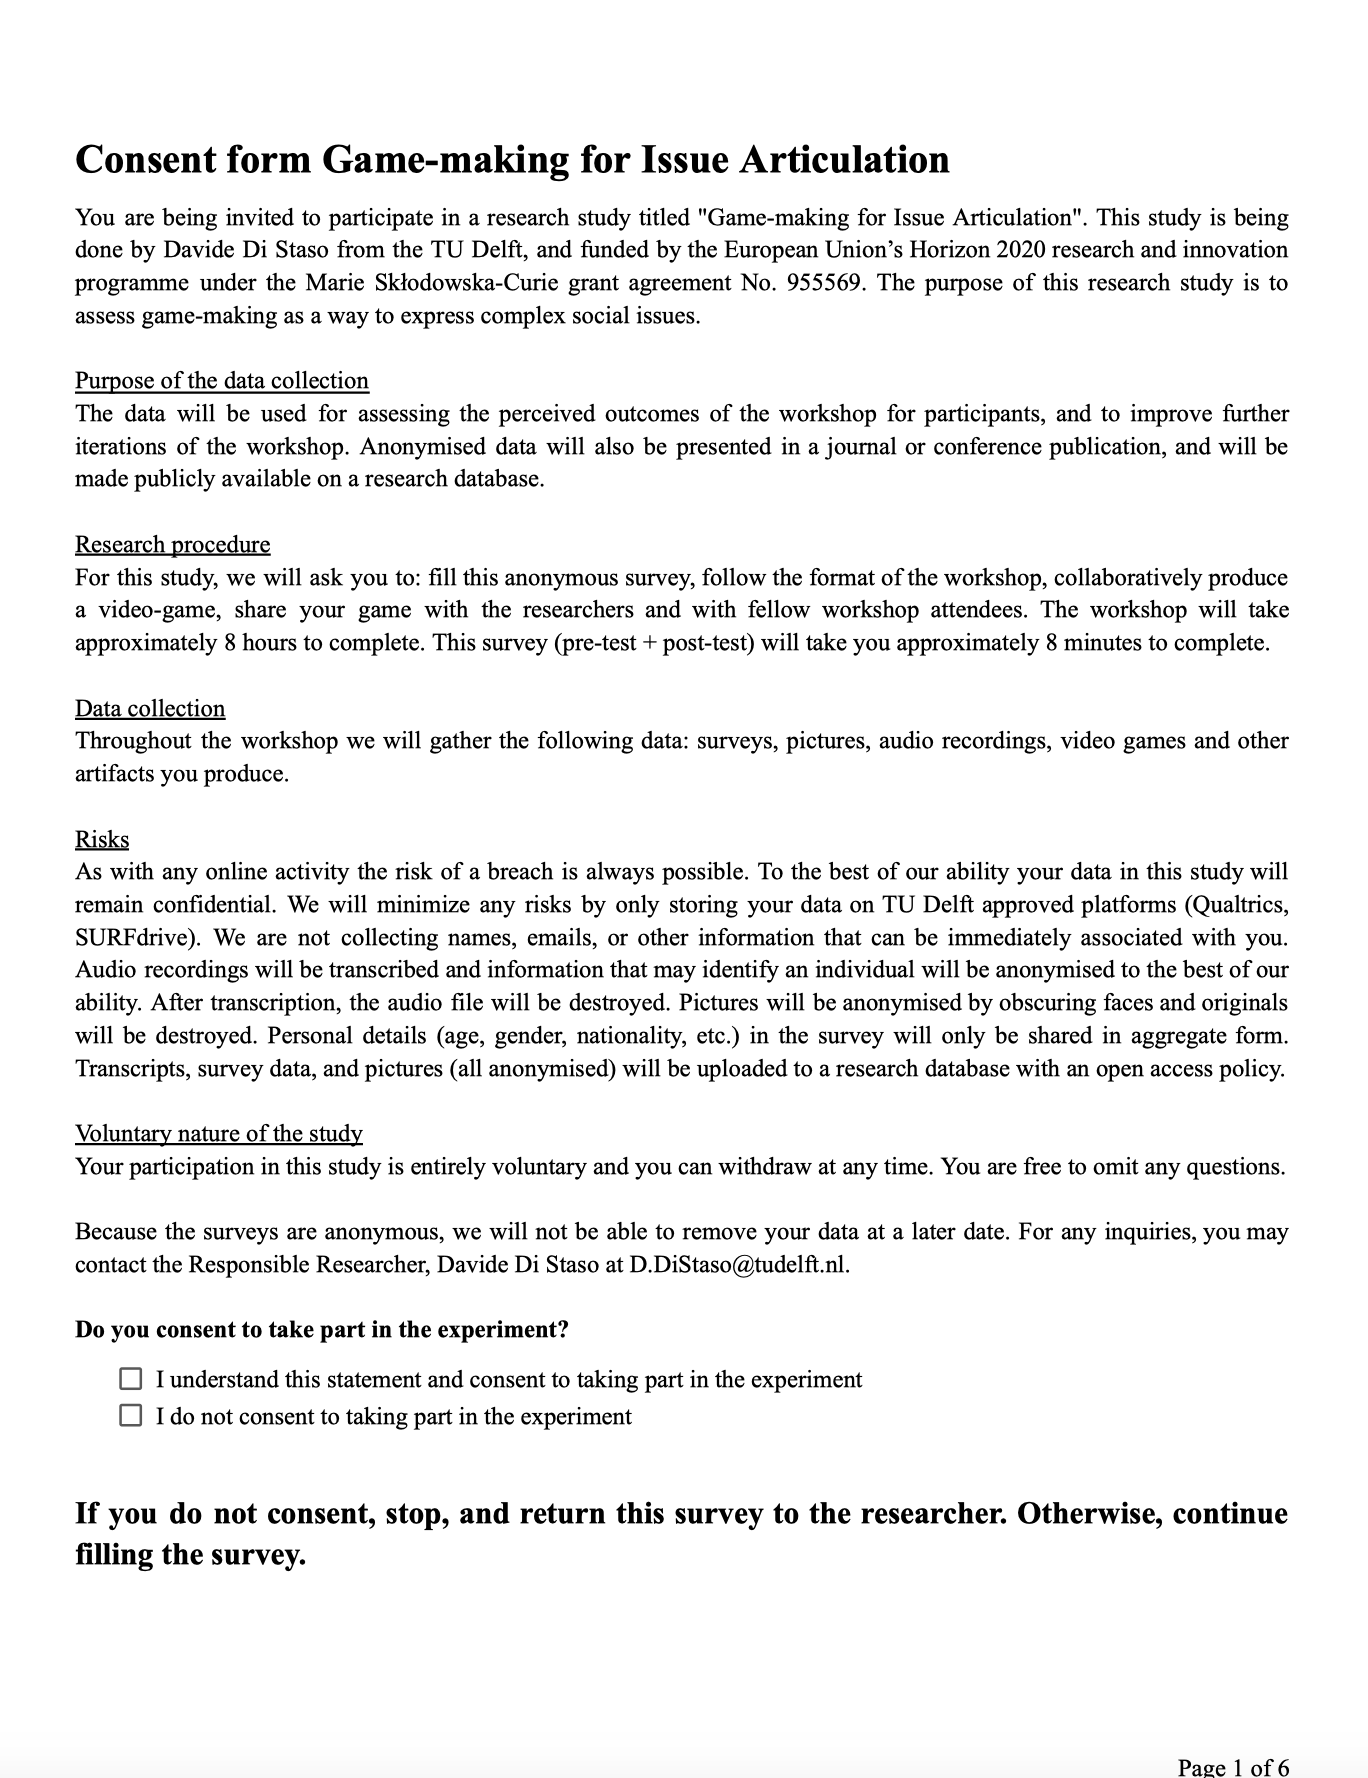
\includegraphics[width=0.8\textwidth]{figures/survey1.png}}
\end{figure}
\end{frame}

\section{Brainstorming}
\begin{frame}
\frametitle{Brainstorming}
Write your game design doc and draw some screenshots
\begin{figure}
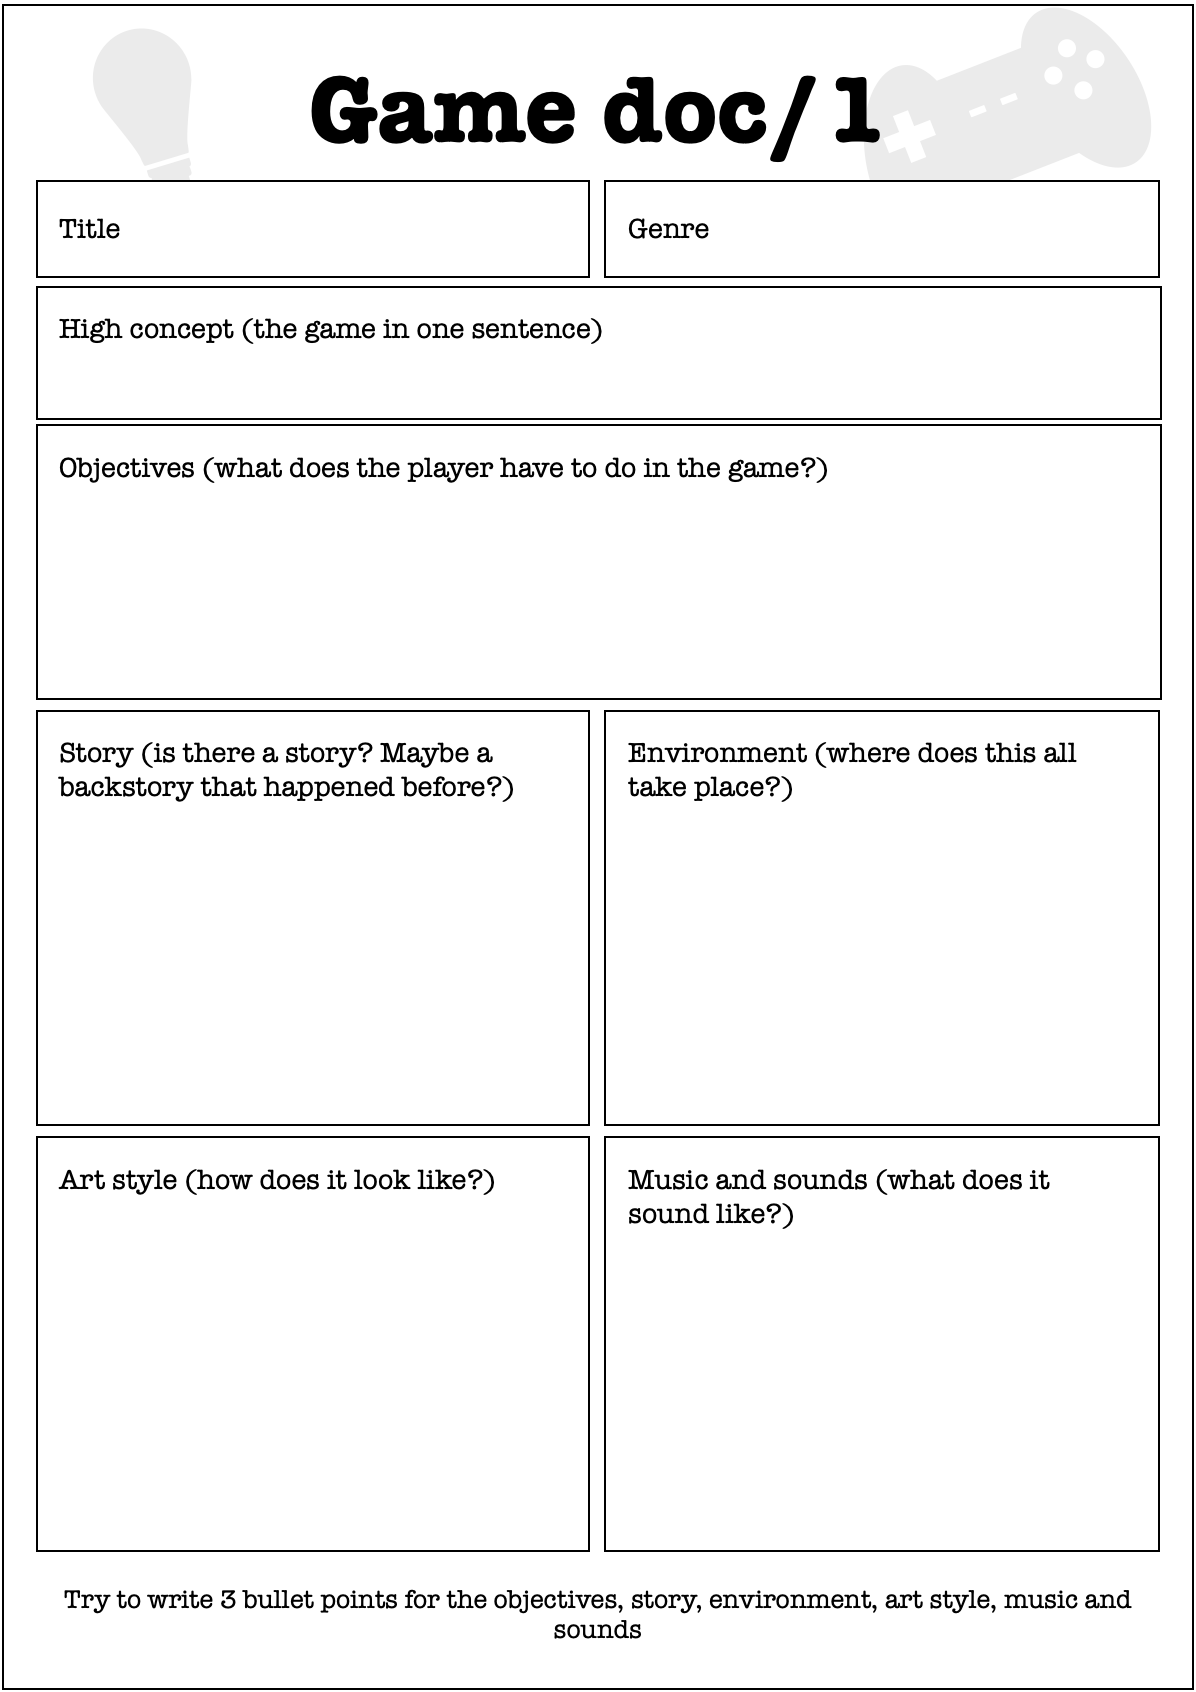
\includegraphics[width=0.3\textwidth]{figures/game_doc1.png}
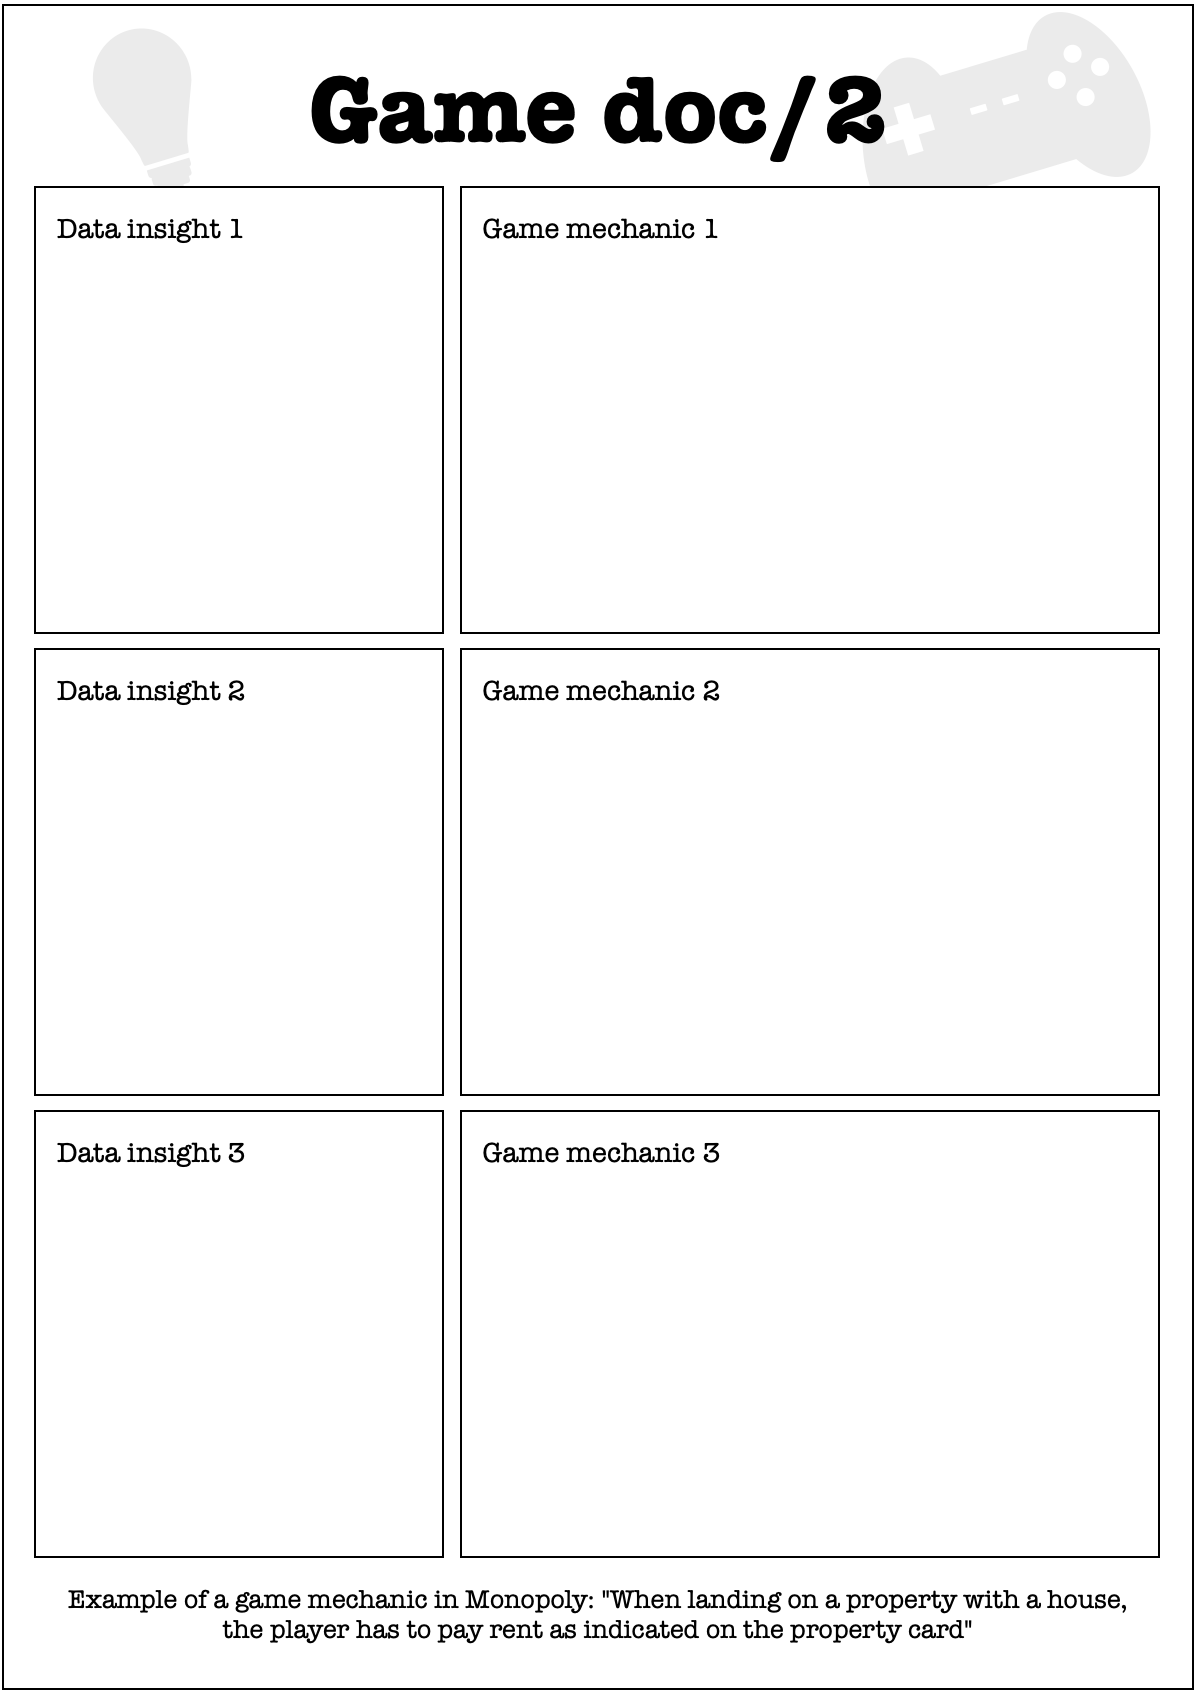
\includegraphics[width=0.3\textwidth]{figures/game_doc2.png}
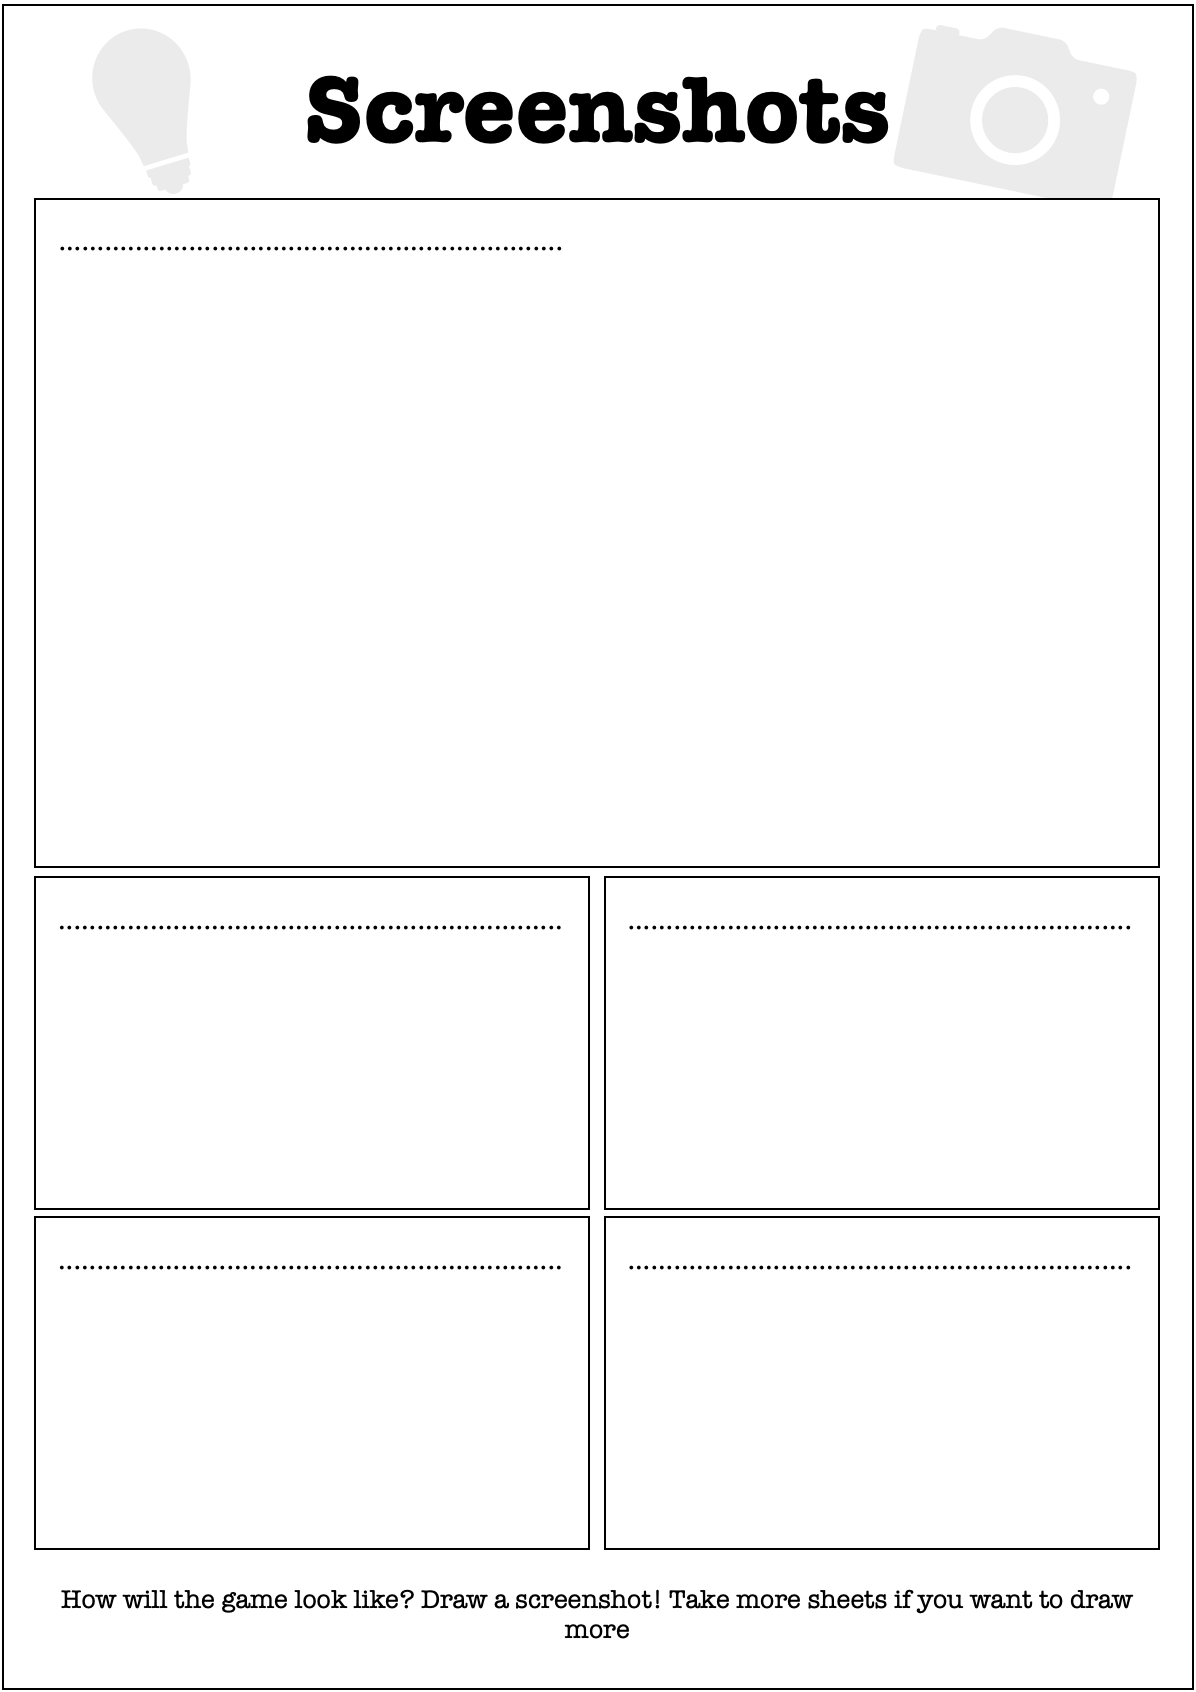
\includegraphics[width=0.3\textwidth]{figures/screenshots.png}
\end{figure}
\end{frame}

\section{Lunch break}
\begin{frame}
\frametitle{Lunch break}
See you in one hour!
\end{frame}

\section{Starter tutorials}
\begin{frame}
\frametitle{Platformer}
\begin{figure}
 \shadowbox{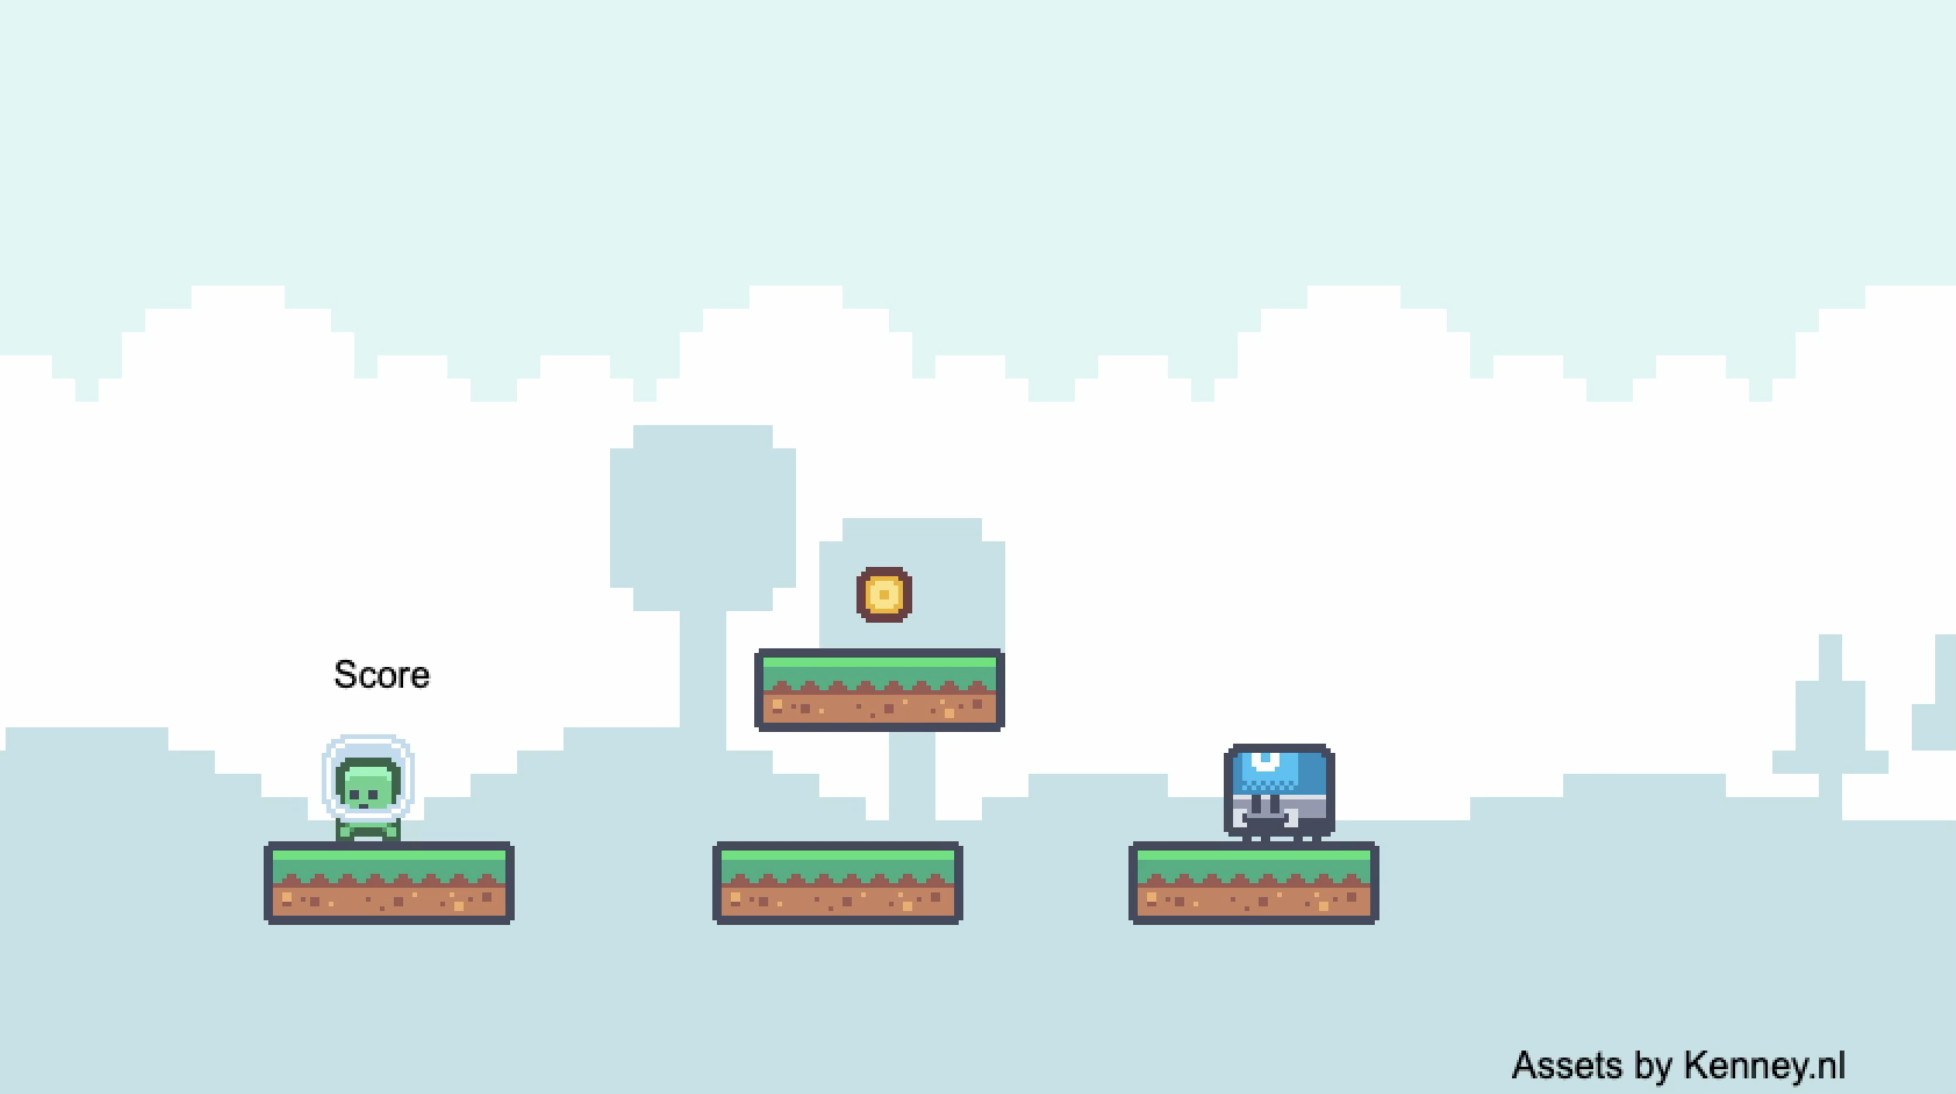
\includegraphics[width=.9\textwidth]{figures/platformer_tutorial.png}}
\end{figure}
\end{frame}

\begin{frame}
\frametitle{Simulation}
\begin{figure}
 \shadowbox{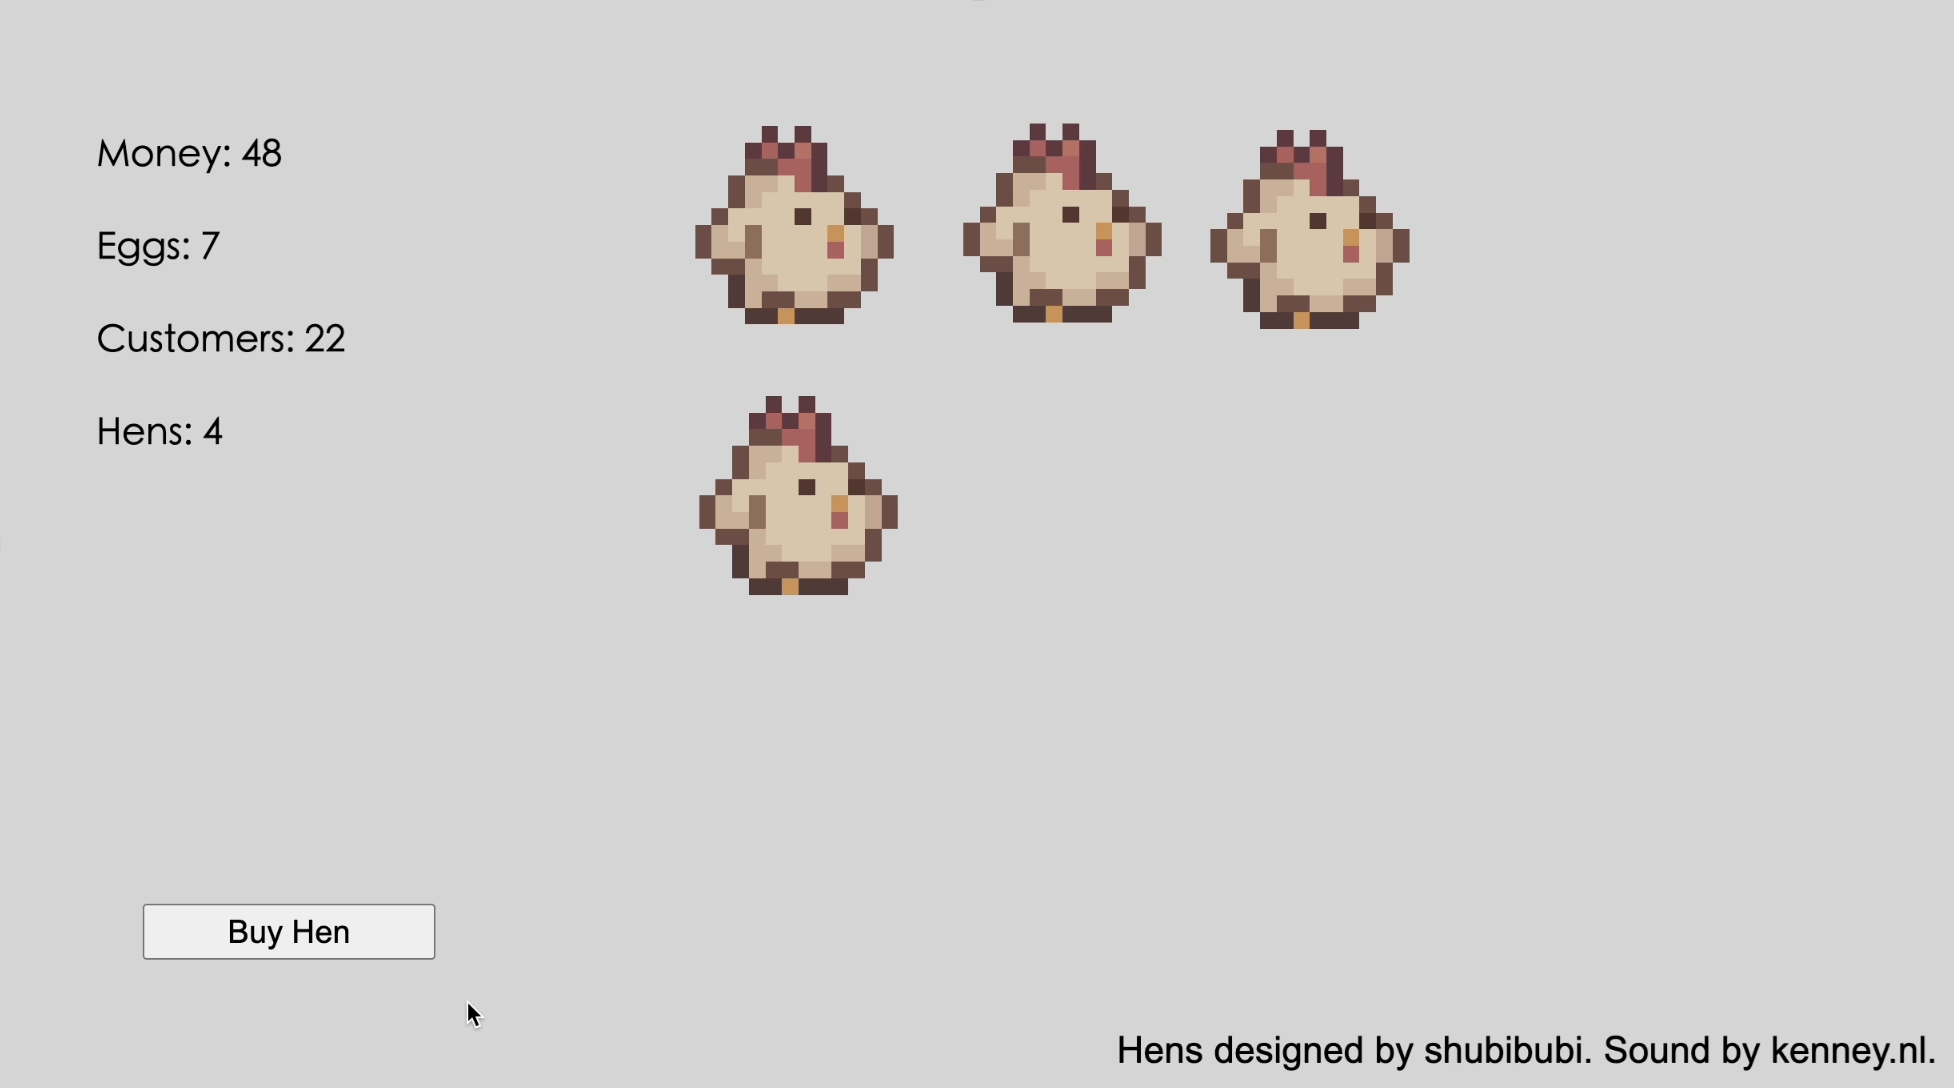
\includegraphics[width=0.9\textwidth]{figures/simulation_tutorial.png}}
\end{figure}
\end{frame}

\begin{frame}
\frametitle{Visual novel}
\begin{figure}
 \shadowbox{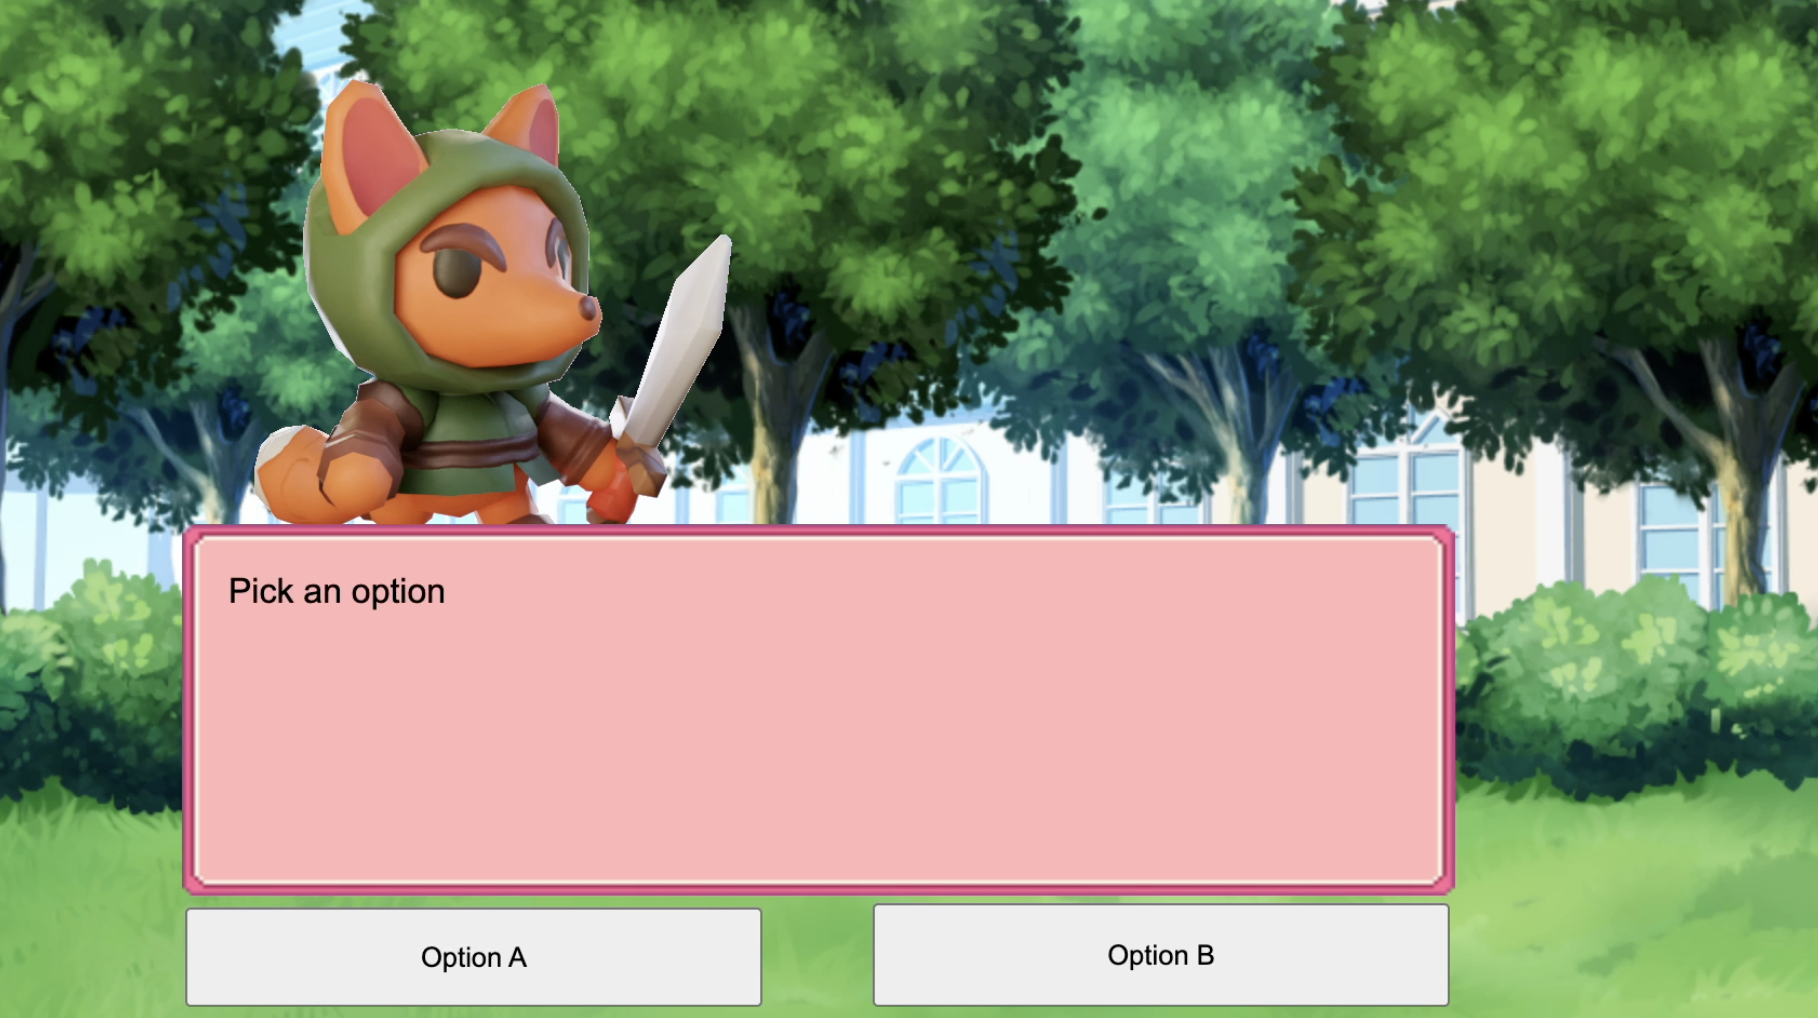
\includegraphics[width=.9\textwidth]{figures/visual_novel_tutorial.png}}
\end{figure}
\end{frame}

\begin{frame}
\frametitle{Check out the starter kits}
https://github.com/davidedistaso/open-data-game-jam
\end{frame}

\section{Coding}
\begin{frame}
\frametitle{Time to code the games}
Feel free to ask for help at any time!
\begin{figure}
\includesvg[width=0.8\textwidth]{figures/coding.svg}
\end{figure}
\end{frame}

\section{Festival}
\begin{frame}
\frametitle{Play each others' games}
And don't forgot to give points to the games you like the most
\end{frame}

\section{Survey section 2}
\begin{frame}
\frametitle{Survey section 2}
Divide into groups of 4
\begin{figure}
 \shadowbox{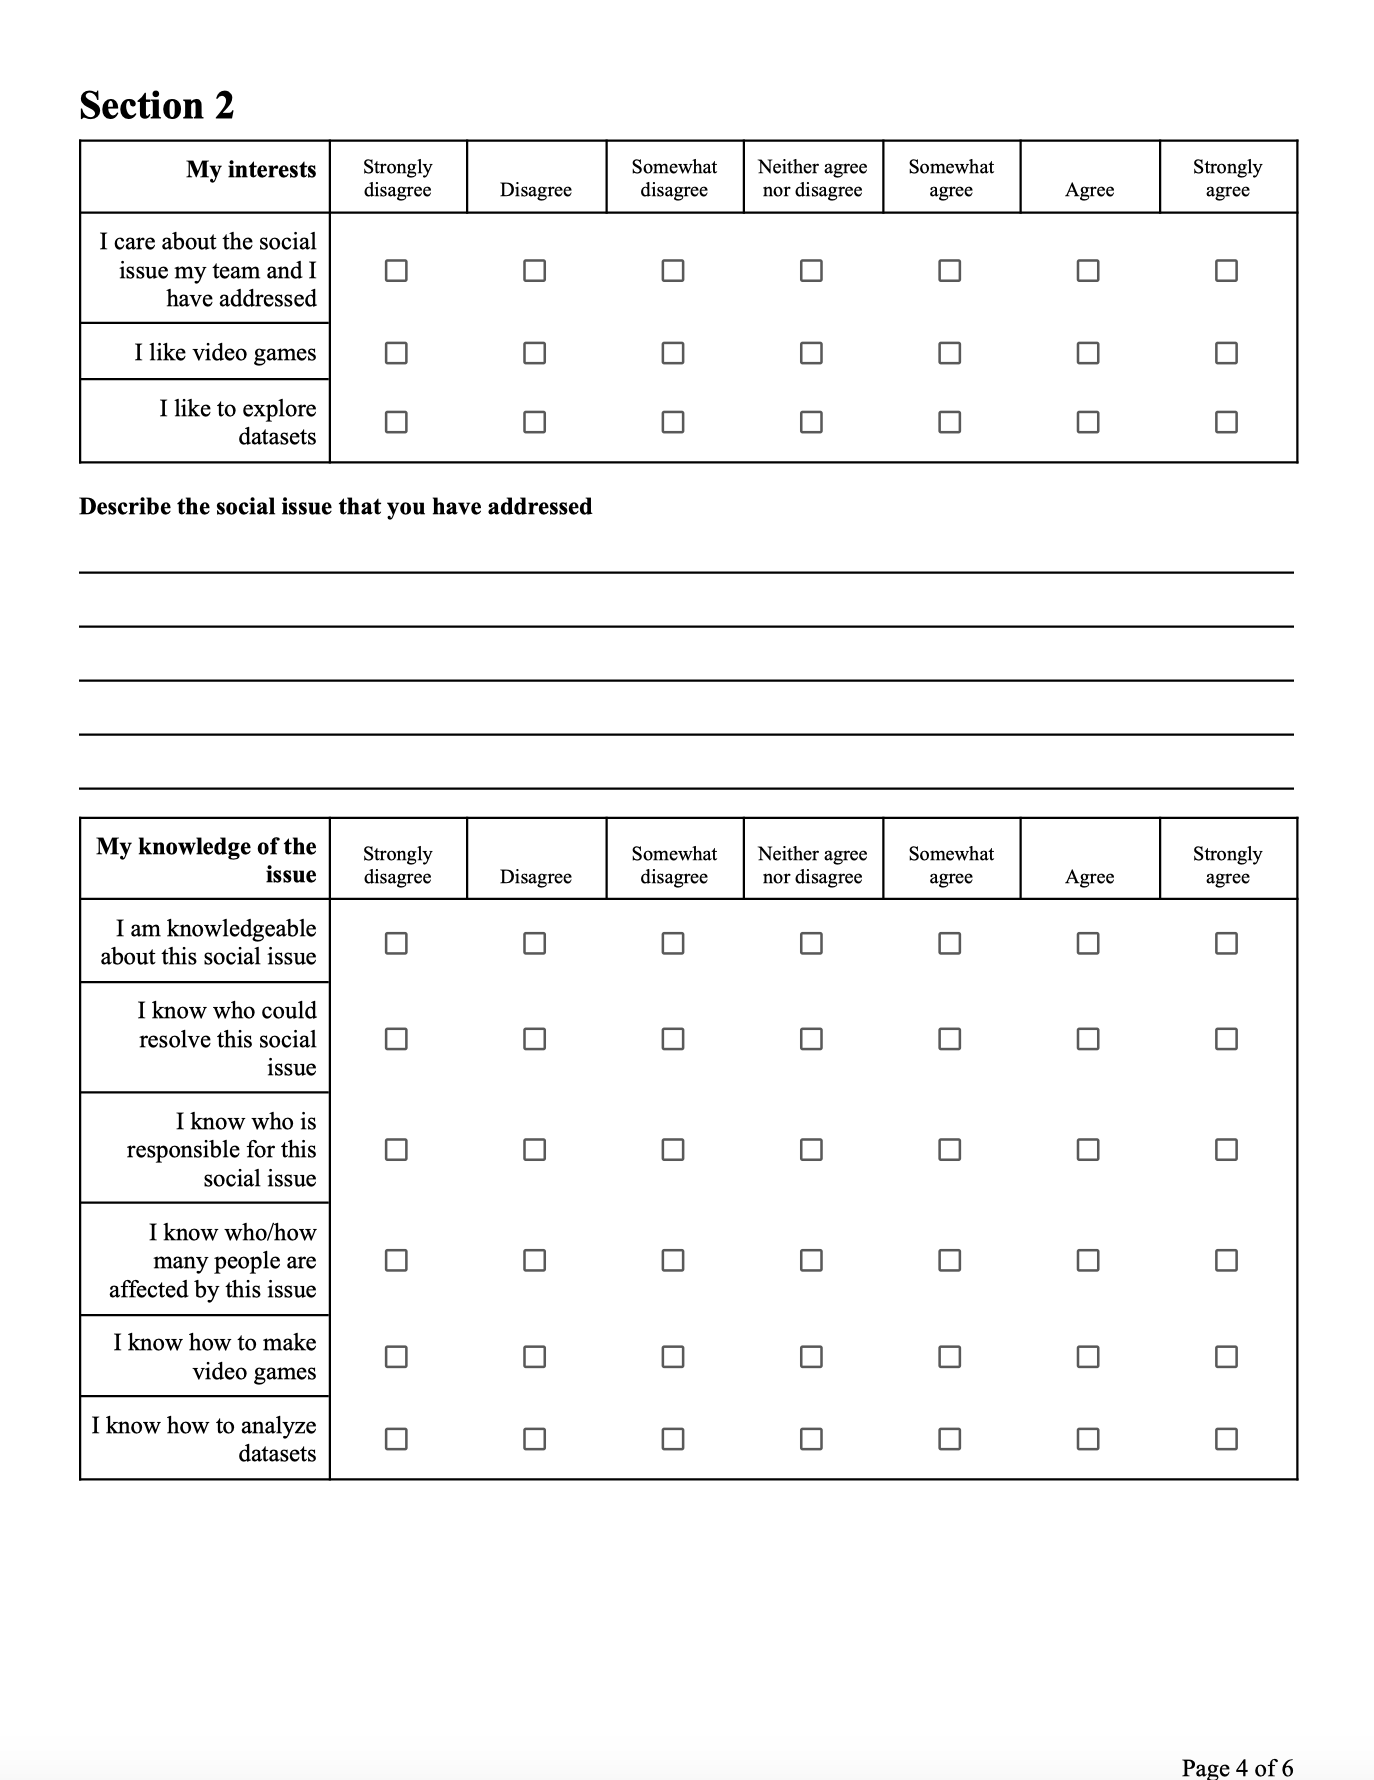
\includegraphics[width=.8\textwidth]{figures/survey2.png}}
\end{figure}
\end{frame}

\section{Winners}
\begin{frame}
\frametitle{Winners}
\begin{figure}
\includesvg[width=0.8\textwidth]{figures/crown.svg}
\end{figure}
\end{frame}

\begin{frame}
Some resources
\frametitle{Want to keep making games?}
\begin{itemize}
    \item https://www.develop.games
    \item Play The Beginner's Guide
    \item D.DiStaso@tudelft.nl
    \item L.V.Christiansen@tudelft.nl
\end{itemize}
\end{frame}
%---------------------------------------------------------


\end{document}